% Configured surface, achieved tool orientation, and physical surface.
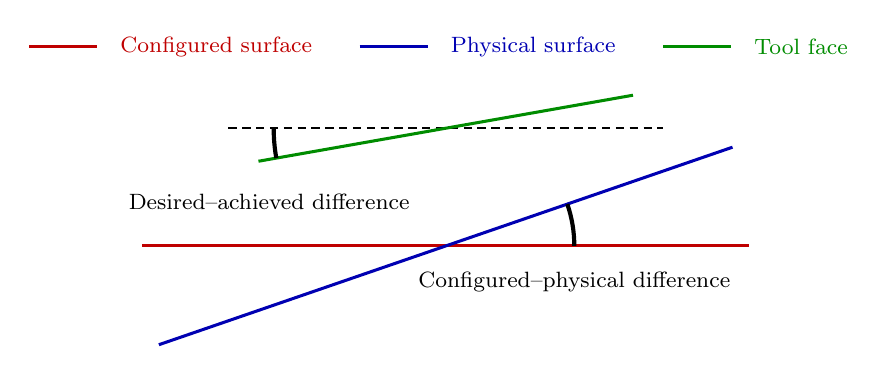
\begin{tikzpicture}[
    scale=1.15,
    reference/.style={red!75!black, line width=1.1pt},
    physical/.style={blue!70!black, line width=1.1pt},
    tool/.style={green!55!black, line width=1.1pt},
    datum/.style={black, line width=0.8pt, densely dashed},
    conceptangle/.style={line width=1.5pt},
    lbl/.style={font=\footnotesize, align=center},
  ]

% Shared legend. The swatch-to-swatch spacing is set so that no entry's text
% reaches the next swatch; check it in the compiled page after any edit.
\draw[reference] (-4.60,2.20) -- (-3.85,2.20);
\node[lbl, red!75!black, anchor=west] at (-3.70,2.20)
  {Configured surface};
\draw[physical] (-0.95,2.20) -- (-0.20,2.20);
\node[lbl, blue!70!black, anchor=west] at (-0.05,2.20)
  {Physical surface};
\draw[tool] (2.40,2.20) -- (3.15,2.20);
\node[lbl, green!55!black, anchor=west] at (3.30,2.20)
  {Tool face};

% The configured surface gives the desired parallel tool direction, carried to
% the tool as a short reference ray. The orientation reached before approach
% retains a small schematic difference from it.
\coordinate (origin) at (0,0);
\coordinate (toolpivot) at (0,1.30);
\draw[reference] (-3.35,0) -- (3.35,0);
\draw[datum] (-2.40,1.30) -- (2.40,1.30);
\draw[tool, rotate around={10:(0,1.30)}] (-2.10,1.30) -- (2.10,1.30);
\begin{scope}[shift={(toolpivot)}]
  \draw[conceptangle]
    (180:1.90) arc[start angle=180,end angle=190,radius=1.90];
\end{scope}
\node[lbl, anchor=north] at (-1.95,0.68)
  {Desired--achieved difference};

% Placement and calibration can leave the physical surface angularly offset.
\draw[physical, rotate around={19:(origin)}] (-3.35,0) -- (3.35,0);
\draw[conceptangle]
  (0:1.42) arc[start angle=0,end angle=19,radius=1.42];
\node[lbl, anchor=north] at (1.42,-0.18)
  {Configured--physical difference};

\end{tikzpicture}
